\subsection{\label{subsec:FZV5}Beugung von Röntgenstrahlen}
\textbf{\textit{a) Was versteht man unter Beugung?}}\\
$\rightarrow$In der Physik bezeichnet der Begriff Beugung das Phänomen, bei dem eine Welle um ein Hindernis oder 
durch eine Öffnung herum abgelenkt wird und sich anschließend in einem bestimmten Muster ausbreitet. 
Dies tritt auf, wenn eine Art von physikalischer Welle auf Hindernisse oder Öffnungen treffen, die in der Größenordnung der Wellenlänge liegen.
Beispiele sind, Lichtbeugung bei Objektiven, die die Auflösungsgrenze bestimmen, Elektronenbeugung an Gitteratomen aufgrund ihrer Welleneigenschaft, 
Schallwellenbeugung, die man täglich wahrnehmen kann und Beugung von Wasserwellen als beispielhaftes Experiment. 
In der Kristallographie wird Röntgenbeugung verwendet, um die Struktur von Kristallen zu analysieren, da die Beugungsmuster Informationen über die 
räumliche Anordnung von Atomen liefert \cite{Schwarz, Kristall}. \\

\textbf{\textit{b) Erklären sie, welche Bedingungen Max von Laue zur Beschreibung der
Röntgenstrahlbeugung heranzog und stellen Sie kurz seinen Ansatz dar!}}\\
$\rightarrow$Die sog.~Laue-Bedingung informiert über das Auftreten von Beugungsreflexen bei der elastischen Streuung von 
Röntgenstrahlung, Elektronen oder Neutronen an Kristallen. Seine Theorie besagt, dass die regelmäßig angeordneten Atome in den 
Kristallen das Röntgenlicht streuen, da die Wellenlänge der Strahlung in der Größenordnung der interatomaren Abstände liegt. 
Der Ansatz beginnt mit einer vereinfacht skalaren Erregerwelle $E(t) = E_{0}e^{-i(\omega_{0}t-\mathbf{k}_{0}\cdot \mathbf{r})}$, 
welche an einem punktförmigen Streuzentrum im Ursprung gebeugt wird. Befindet sich ein anderes Streuzentrum bei $\mathbf{R}$, so gilt 
für die Phasenbeziehung der gebeugten Kugelwellen $\Delta\Phi = (\mathbf{k} - \mathbf{k}_{0})\cdot \mathbf{R}$. Geht man von einer 
ausgedehnten Probe aus, so muss über die Gesamtheit der Streudichte summiert bzw.~über eine Streudichte $\rho(\mathbf{r})$ integriert werden.
Für die gestreute Welle gilt
\begin{equation}\label{eq:streu}
    E_{\text{S}}(t) = \frac{\tilde{E}}{R}e^{-i(\omega_{0}t-k_{0}R)}\int_{V_{\text{Kristall}}}\,\rho(\mathbf{r})e^{-i \mathbf{K}\cdot \mathbf{r}}\,dV,
\end{equation}
wobei $\mathbf{K} = \mathbf{k} - \mathbf{k}_{0}$ also Streuvektor eingeführt wird. Bis auf Vorfaktoren erhalten wir folglich die gemessene Intensität 
im Abstand $R$ als Funktion des Streuvektors durch betragliche Quadration von Gl.~\eqref{eq:streu}. Nutzt man aus, dass die (zeitlich gemittelte) Streudichte
periodisch ist, so kann diese als Fourier-Reihe dargestellt werden, die die reziproke Darstellung des Gitters und damit die Miller'schen Indizes inkludiert. 
Für die gemessene Intensität in Abhängigkeit des Streuvektors gilt
\begin{align}
    I(\mathbf{K}) &\propto \left\vert\sum_{h,k,l}\rho_{hkl}\int_{V_{\text{Kristall}}}\,e^{i(\mathbf{G}_{hkl}-\mathbf{K})\cdot\mathbf{r}}\right\vert^{2} \label{eq:laue}\\
    \mathbf{G}_{hkl} &= h\tilde{\mathbf{a}} + k\tilde{\mathbf{b}} + l\tilde{\mathbf{c}} \\
    \tilde{\mathbf{a}} &= \frac{2\pi}{V_{\text{primitive Elementarzelle}}}(\mathbf{b}\times \mathbf{c})\hspace{0.5cm}\text{und zyklisch}.
\end{align}
Hierbei sind $h,k,l$ die Miller-Indizes, $\mathbf{G}_{hkl}$ bezeichnet den reziproken Gittervektor, der von den reziproken Basisvektoren 
erzeugt wird und $\rho_{hkl}$ sind die Fourier-Koeffizienten der Streudichte. \\
Das Integral mittelt sich weg, falls $\mathbf{G}_{hkl}\neq \mathbf{K}$, was uns schlussendlich zur Laue-Bedingung führt
\begin{equation}
    \fbox{$\mathbf{G}_{hkl} = \mathbf{K}$},
\end{equation}  
welche besagt, dass die Änderung des Wellenvektors einem reziproken Gittervektor entsprechen muss, damit konstruktive Interferenz sichtbar wird. 
Außerdem sieht man, dass die detektierte Intensität proportional zum Betragsquadrat des Fourier-Koeffizienten $\rho_{hkl}$ ist \cite{EPC}. \\

\textbf{\textit{c) William Henry Bragg und sein Sohn William Lawrence Bragg verwendeten
ein komplett anderes aber äquivalentes Modell zur Beschreibung der
Röntgenstrahlbeugung. Erläutern Sie dieses! Wie lautet in diesem Kontext
die Braggsche Gleichung? Welchen physikalischen Zusammenhang
stellt sie dar? Erklären Sie diesen Zusammenhang anschaulich!}}\\
$\rightarrow$Die Bragg-Theorie nimmt hingegen an, dass die Kristallatome Ebenen im Abstand $d$ bilden, an denen die 
einfallenden Röntgenstrahlen teilweise reflektiert werden. Hierdurch entstehen Teilstrahlen, die je nach Einfallswinkel eine
bestimmte Phasendifferenz aufweisen. Ist diese Phasendifferenz ein ganzzahliges Vielfaches der eingestrahlten Wellenlänge, 
so interferieren die Teilstrahlen konstruktiv und es entsteht ein Peak auf dem Detektorschirm. Mittels geometrischer Überlegungen, 
die in Abb.~\ref{fig:bragg} dargestellt sind, folgt die Braggsche Gleichung zu
\begin{equation}\label{eq:bragg}
    \fbox{$n\lambda = 2d\sin(\Theta)$},
\end{equation} 
wobei $n$ die Beugungsordnung, $\lambda$ die Wellenlänge (Röntgenstrahlung oder Materiewelle) und $\Theta$ der Einfallswinkel zur betrachteten 
Gitterebene ist. Für den Abstand der Gitterebenen gilt $d = 2\pi/|\mathbf{G}_{hkl}|$.
\begin{figure}[h!]
    \centering
    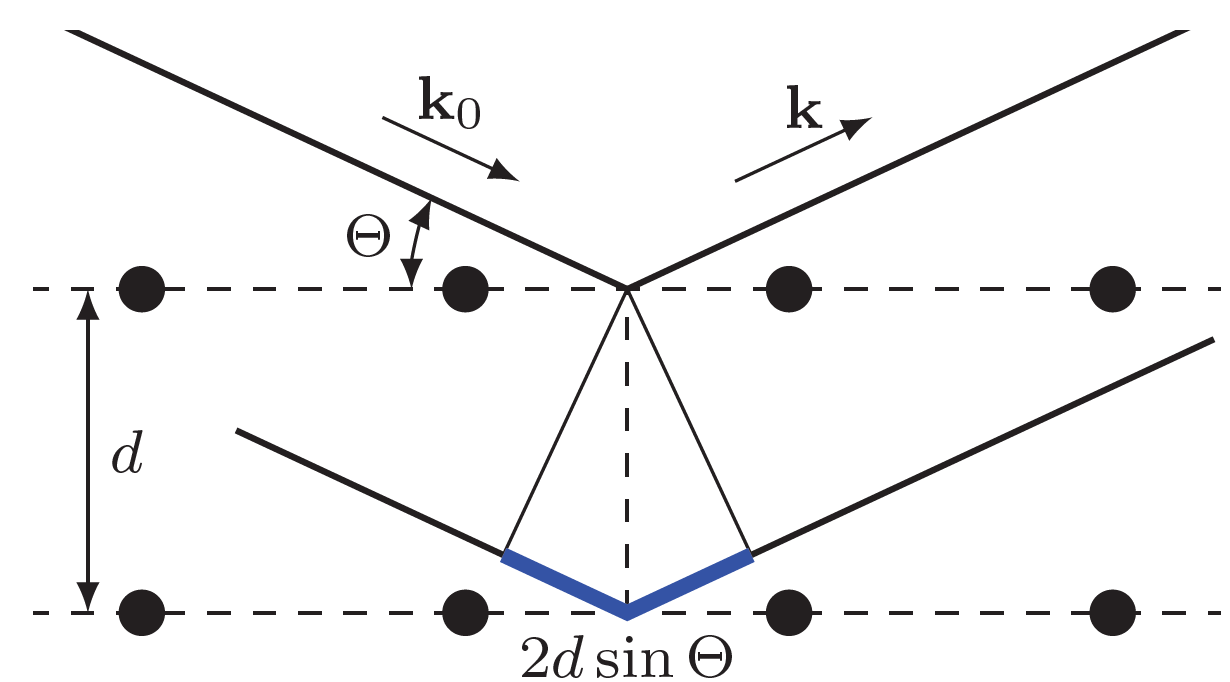
\includegraphics[width=0.44\textwidth]{Braggi.png}
    \caption{\label{fig:bragg}Skizzenhafte Darstellung der an zwei Gitterebenen reflektierten Teilstrahlen, sowie 
    die berechnete Wegdifferenz (blau).}
\end{figure}\FloatBarrier \,\newpage
Die Beugungsbedingungen von Laue und Bragg entstehen aus zwei komplett unterschiedlichen Ansätzen, lassen sich aber ineinander überführen. 
Für den Betrag des Streuvektors gilt allgemein aus geometrischen Überlegungen der Reflexion $|\mathbf{K}| = \frac{4\pi}{\lambda}\sin(\Theta)$, 
zudem gilt $|\mathbf{G}_{hkl}| = \frac{2\pi}{d}$, woraus mit der Laue-Bedingung $\mathbf{G}_{hkl} = \mathbf{K}$ direkt die 
Bragg'sche Gleichung folgt \cite{EPC}. \\

\textbf{\textit{d) Hält man einen Einkristall in einen monochromatischen Röntgenstrahl,
so passiert normalerweise nichts. Welche Bedingung muss erfüllt sein, damit
ein Beugungsreflex entsteht? Welche beiden Parameter kann man nun
variieren, damit man an diesem Einkristall einen Beugungsreflex erfassen
kann?}}\\
$\rightarrow$Mit Gl.~\eqref{eq:bragg} wird klar, dass bei monochromatischem Licht einer Wellenlänge
$\lambda_{0}$ nur Reflexe detektiert werden, wenn für den 
Einfallswinkel $\Theta = \arcsin(n\frac{\lambda_{0}}{2d})$ gilt. Das es gerade eine Schar von Gitterebenen 
gibt, die bei eingestelltem $\Theta$ den gewünschten Abstand $d$ hat, ist unwahrscheinlich, weswegen 
normalerweise kein Signal detektiert wird (nichts passiert).
Durch gezielte Variation der Wellenlänge und des Einfallswinkels zur Kristalloberfläche 
kann man also die Bedingungen für konstruktive Interferenz erfüllen und Beugungsreflexe 
an einem Einkristall erzeugen. 
Dies wird in der Röntgenkristallographie und anderen Methoden der Festkörperanalyse genutzt, 
um Informationen über die Kristallstruktur zu erhalten.
